\documentclass[tikz,multi,border=10pt]{standalone}
\usetikzlibrary{arrows.meta,shadows,positioning}
\usepackage{enumitem}
\usepackage{courier}
\renewcommand*\familydefault{\ttdefault}
\begin{document}
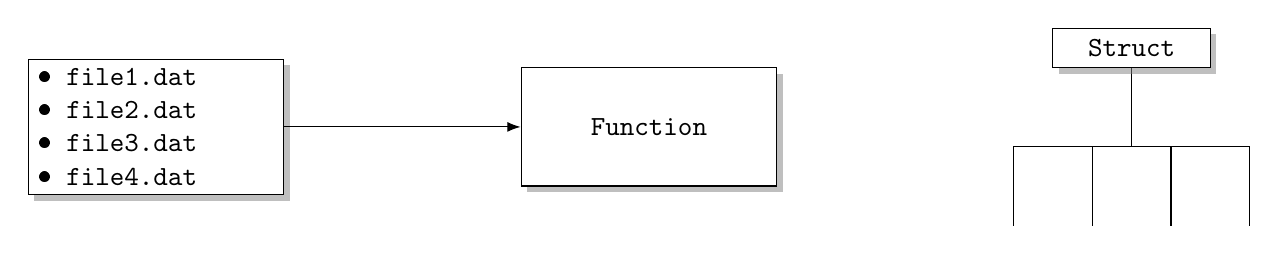
\begin{tikzpicture}
  [
    node distance=3cm,
    basic/.style={%
      draw, fill=white
    },
    files/.style = {%
      basic,
      text width=3cm,
      minimum height=1.5cm
    },
    function/.style = {%
      basic,
      text width=3cm,
      minimum height=1.5cm,
      text centered
    },
    box/.style = {%
      basic,
      minimum width=2cm,
      minimum height=0.5cm
    },
    arrow/.style={%
      ->, >=Latex,
    },
  ]
  \begin{scope}[local bounding box=output]
    \draw (0,0) -- (0,1) node[above, box, drop shadow] {Struct};
    \draw (-1.5,-1) -- (-1.5,0) -- (1.5,0) -- (1.5,-1);
    \draw (-0.5,-1) -- (-0.5,0);
    \draw (0.5,-1) -- (0.5,0);
  \end{scope}
  \node (function) [function, left= of output, drop shadow] {Function};
  \node (files) [files, drop shadow, left=of function,] {%
    \vspace*{-.5\baselineskip}%
    \begin{itemize}[nosep,leftmargin=*]
      \item{file1.dat}
      \item{file2.dat}
      \item{file3.dat}
      \item{file4.dat}
    \end{itemize}
  };
  \draw [arrow] (files) -- (function);
\end{tikzpicture}
\end{document}
